\chapter{Fake News: An Inquiry}

\begin{abstract}
We present an analysis of various fake news datasets and evaluate various classification tasks. We compare the different types and sources of information, analyze their characteristics, and show how the state-of-the-art text classification techniques can improve the fake news detections. To investigate the scope of the fake news, we choose various types of text datasets, ranging from satire, hoax, propaganda, fact-checked political statements, and trustworthy news articles, and show that the classifiers can discriminate the underlying structure of these sources. Experimental results suggest that while in-domain fact-checking and truthfulness judgments can be achieved, identifying nuances and out-of-domain cases remains an open research question.
\end{abstract}

\section{Introduction}
The term "fake news" is rather a new term in our social and political discourse. The effect of fake news was highlighted during the U.S presidential election in 2016, where the two parties accused each other and the media to engage in spread falsehood against each party. The term fake news can be used to describe a wide range of information, from satirical articles to complete fabrication of a story. The fake news problem grows as the spread of (mis)information becomes easier and cheaper with the social media, and more severely affect the society as the individuals become trapped in their social network echo chambers. We need first to have an understanding on what constitutes fake news become we can attempt to find a remedy in fields of machine learning (ML), natural language processing/understand (NLP/NLU), and artificial intelligence (AI). 

Generally speaking, we can define fake news as a fabricated story with the intention to deceive \footnote{\url{https://www.nytimes.com/2016/12/06/us/fake-news-partisan-republican-democrat.html}}. There are two key points in this view of fake news, first is the intentionality to deceive (which is rather a difficult task in NLU), and second, that story is fabricated and therefore should fail the fact-checking. The proof of intent to deceive is very vague even for many human subjects, and that makes it even hard to define it as an NLU task. 

To be more pragmatic, we can describe the fake news problem domain with following challenges\footnote{\url{https://miguelmalvarez.com/2017/03/23/how-can-machine-learning-and-ai-help-solving-the-fake-news-problem/}}: fact-checking, source credibility and trust, news bias, and misleading headlines. There are many fact-checking initiatives to alleviate the problem of fake news. Websites like politifact.com and factcheck.org aim to provide factual check of the politicians' statements. The specialized curated list of online sources, such as OpenSources \footnote{\url{http://www.opensources.co/}} provide trustworthy sources of information for online users.  In recent years,  ML communities like Fake News Challenge (FNC) \footnote{\url{http://www.fakenewschallenge.org/}} has taken on the issue of stance detection, which aims to evaluate the misleading headlines and the article bodies. In this research, we take a look at the nature of fake news by evaluating the ML and NLU techniques and the available datasets.

Our primary contribution is to analyze various fake news datasets and report state-of-the-art classification performance baselines for these datasets. The motivation is behind this approach is twofold: first is to set higher baselines for the fake news classification, and second to raise the need for more comprehensive and representative datasets.  


\section{Evaluating Truthfulness}
In this work, we focus on presenting various available fake news datasets and analyze the performance of state-of-the-art classification techniques.   

\citet{Kim14convolutionalneural} proposed an effective convolutional neural network for the sentence classification. The CNN architecture is inspired by high-dimensional computer vision classification problem. We experimented with various variants of the model (CNN-Rand, CNN-static, CNN-non-static), and finally chose the CNN-static, which has pre-trained vectors from \texttt{word2vec} \footnote{\url{https://code.google.com/p/word2vec/}} word embedding, to be the best suiting for our classification task.

The bidirectional GRU \cite{DBLP:journals/corr/BahdanauCB14},  are composed of two independent RNNs together, in this case Gated Recurrent Unit (GRU) \cite{ChoMGBSB14}. The bidirectional GRU contains a forward GRU $\overrightarrow{f} $ which reads the sentence as a forward sequence, and backward GRU $\overleftarrow{f}$ which read the sequence in reverse. This property of bidirectional GRU model allows the model to encode the contextual information of the text.

In GRU-2 model \cite{Ma2016DetectingRF}, there are two GRU hidden layers and embedding layer, that is able to capture higher-level features of the text.  We also explore the performance of hierarchical attention network \cite{Yang2016HierarchicalAN} for the fake news classification (Figure \ref{fig:HAN}). The model has four main components, word sequence encoder, a word-level attention layer, a sentence encoder and a sentence-level attention layer. Lastly, we examine the performance of the fastText \cite{DBLP:journals/corr/JoulinGBM16}, a simple and highly efficient approach built on top of a linear model with rank constraint and optimized loss approximation.  

\begin{figure}[!ht]
\centering
\caption{\small{Hierarchical Attention Network \cite{Yang2016HierarchicalAN}}}
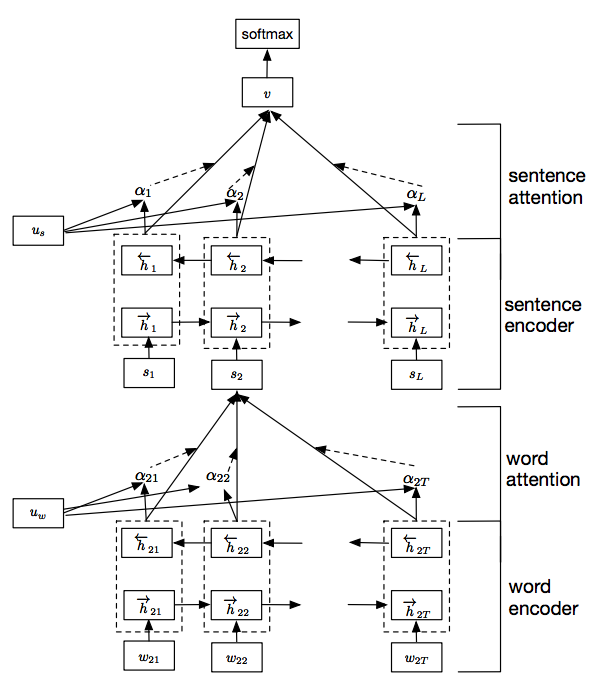
\includegraphics[scale=.5]{img/HierachicalAttention}
\label{fig:HAN}
\end{figure}

\section{Experiments}

\subsection{Datasets}
\textbf{Unreliable News Dataset} \cite{Rashkin2017TruthOV} is a news article dataset that takes various type of information, ranging from trusted, satire, hoax to propaganda into consideration (See Table \ref{table:Unreliable_News_Dataset}). The various types of news sources in this dataset provide a rich environment for classification task and analyzing the lexicon and semantic differences of these news sources.   

\textbf{FakeNewsNet} is a dataset curated by \citet{shu2018} which contains publishers, news content and social engagement information. The dataset is based on the news vendor BuzzFeed and fact-checking website PolitiFact. To simplify the task, and avoid trivial classification solution, the dataset is divided into balanced True and False categories.   

\textbf{PolitiFact} we curated from the politifact.com and analyze the feasibility of the discerning facts from fiction. Politifact evaluates each statement in a 6-point scale of truth value, ranging from "True" to "Pants on Fire!". We collected 14,397 statements from 3,806 different individuals for the experiments and assigned binary categories of True/False to each record. 

\textbf{Snopes.com} is among one the oldest rumors and fact-checking services on the web. They investigate a range of claims, from urban legends, myths, to fake news and political statements. Similar to PolitiFact, they use scale points ranging from true, mostly true to unverified and false to evaluate each story. To build the dataset, we crawled all the fact-checked stories on Snopes.com, and assign the True or False labels to the claims. All datasets described here are publicly available for fake news research\footnote{Available at \url{http://annonomized}}. 
 
\begin{table*}[!ht]
\centering
  \caption{Classification performance results}
  \label{table:result}
\resizebox{\textwidth}{!}{%
\begin{tabular}{lcccccccc}
\toprule
\textbf{Dataset} & \multicolumn{2}{c}{\textbf{PolitiFact}} & \multicolumn{2}{c}{\textbf{Unreliable News}} &  \multicolumn{2}{c}{\textbf{FakeNewsNet}} & \multicolumn{2}{c}{\textbf{Snopes}} \\
\cmidrule(lr){2-9}
\textbf{Metric} & {Accuracy} & {F1-score} & {Accuracy} & {F1-score} & {Accuracy} & {F1-score} & {Accuracy} & {F1-score}  \\
\midrule
\texttt{LR}  &$0.579$ 	& $0.578$ & $0.954$ & $0.955$ &	$0.819$ & $0.819$ & $\textbf{0.813}$ & $0.747$ \\
\texttt{PAC}  &$0.552$ 	& $0.553$ & $0.967$ &  $0.967$	 &	$\textbf{0.833}$ & $\textbf{0.833}$  & $0.793$ & $\textbf{0.755}$ \\
\texttt{SVM(Linear)}  &$0.601$ 	& $0.598$ & $0.963$ &  $0.963$	& $0.828$	&  $0.828$  &  $0.789$ & $0.753$ \\
\midrule
\texttt{GRU-2}  	&$0.603$ 	& $0.604$	& $\textbf{0.975}$ & $0.949$  & $0.595$	 & $0.596$ &  $0.799$ & $0.710$  \\
\texttt{bi-GRU}  	&$0.581$ 	& $0.582$	& $0.945$ & $0.945$ &	$0.654$ & $0.637$  &  $0.792$ & $0.732$\\
\texttt{Yoon-CNN}  	&$0.597$ 	& $0.592$	& $0.939$ & $0.939$ &	$0.738$ &  $0.729$   &  $0.798$ & $0.710$ \\
\texttt{FastText}  	& $\textbf{0.632}$ 	& $\textbf{0.632}$	& $0.968$ & $0.951$ &	$0.702$ &  $0.713$   &  $0.799$ & $0.710$ \\
\texttt{HAN}  		&$0.580$ 	& $0.579$	& $0.973$ & $\textbf{0.974}$ & $0.750$	 & $0.750$  &  $0.753$  & $0.733$ \\
\bottomrule             
\end{tabular}
}
\end{table*}


\begin{table}[!ht]
\centering
  \caption{Unreliable News Dataset \citet{Rashkin2017TruthOV}}
  \label{table:Unreliable_News_Dataset}
\resizebox{.5\columnwidth}{!}{%
  \begin{tabular}{lcc}
  \toprule
  \textbf{Statistic} & Source & {\# of Docs}   \\
  \midrule
  \textbf{Trusted}  & Gigaword News & $13,995$ \\
  \midrule
  \textbf{Satire} & \shortstack{The Borowitz Report \\ The Onion \\ Clickhole}  &  $14,985$\\ 
  \midrule
  \textbf{Hoax} & \shortstack{American News \\ DC Gazette} & $12,047$  \\ 
  \midrule
  \textbf{Propaganda} & \shortstack{The Natural News \\ Activist Repost} &  $33,449$\\ 
  \bottomrule             
  \end{tabular}
}
\end{table}


\subsection{Experimental Settings}
We use various baseline techniques and evaluate their performance on different fake news dataset. The following methods are used: logistic regression classifier (LR), Passive Aggressive Classifier (PAC) \cite{Crammer:2006:OPA:1248547.1248566}, support vector machine classifier (SVM-Linear) \cite{Crammer:2002:AIM:944790.944813}, a bi-directional GRU model (Bi-GRU),  GRU-2 model \cite{Ma2016DetectingRF}, Hierarchical Attention Network (HAN) \cite{Yang2016HierarchicalAN}, and convolutional neural network model (CNNs) \cite{Kim14convolutionalneural}. 

We tokenized all texts in experiments with NLKT \footnote{\url{https://www.nltk.org/}} and used Scikit-learn library \footnote{\url{http://scikit-learn.org/stable/}} to implement the baseline classifiers. Deep learning models are implemented in Keras\footnote{\url{https://keras.io/}} library in Python. For the neural network models, we used pre-trained GloVe \cite{pennington2014glove} word embedding trained on Common Crawl with 840 billion tokens.  Deep learning models are run on Quadro P5000 16GB GPUs.

\section{Results and discussion}
FakeNewsNet has a balanced number of fake and real news; however, the total number of records (422 news articles) makes the dataset very limiting for exploring deep learning solutions. The results from our experiments show that the performance of deep learning methods (GRU-2, Bi-GRU, Yoon-CNN, and HAN) suffer significantly on this dataset, which we believe is due to lack of enough training data. We should also note that the traditional baselines such as SVM perform better than most feature engineered baselines reported by \citet{shu2018}.  

We also observed that all of the classification methods presented outperform the lexicon feature engineered approach presented in \citep{Rashkin2017TruthOV}. This is due to the fact that the \citet{Rashkin2017TruthOV} chose a weak baseline (random guess) to compare their feature engineered classifiers.  


\section{Related Work}
Researchers have focused on different aspects of fake news problem. \citet{Rashkin2017TruthOV} focused on the linguistic analysis of the news media and showed that the stylistic feature of the text could help to determine the truthfulness of the news. Drawing on the Linguistic Inquiry and Word Count (LIWC) \cite{Pennebaker}  on psychometric properties of lexicons, authors showed that different types of information (satire, hoax, propaganda) exhibits distinguishable lexicons that can improve the classification task. \citet{fourney_cikm2017} took the approach of analyzing the traffic of websites known for publishing fake news during the 2016 US presidential election. Based on the user browsing history, they observed that certain stories continue to persist in circulation, while others are short-lived and disappear after few days. 

To detect the temporal spread of rumors in microblogs, \citet{Ma2016DetectingRF} combined RNN-based methods with variable-length time series approach to analyzing the microblog posts. By utilizing the variations of aggregated information across different time intervals, this work focuses on the temporal spread of rumors in social media and detect rumors in the early stages. Similarly, \citet{Wu_rumors} and \citet{Sampson:2016:LIS:2983323.2983697} proposed methods to track rumors by collecting and filtering posts related specific rumors and classify the relevance (stance) of the post to the rumor's veracity (truthfulness). 

Clickbaits create a curiosity gap by eye-catching headlines in online media. Clickbaits are ideal form for the spread of fake news since they increase the likelihood that the reader will hit the target link to get exposed to the information. An approach is taken by Fake News Challenge and Clickbait Challenge \footnote{\url{https://www.clickbait-challenge.org/}} is to detect the stance of media headlines with the content to evaluate the trustworthiness of the source \cite{RiedelASR17, Cao2017MachineLB, Zeng2017NeuralSD}.

\section{Conclusion}
We provided an analysis of various available fake news datasets and evaluated baseline and state-of-the-art classification task techniques. We are aware of the imperfection of this work, and encourage the research community to address the inherit shortcomings that stem from limited representative datasets.    
